% Created by tikzDevice version 0.10.1 on 2018-01-23 02:21:11
% !TEX encoding = UTF-8 Unicode
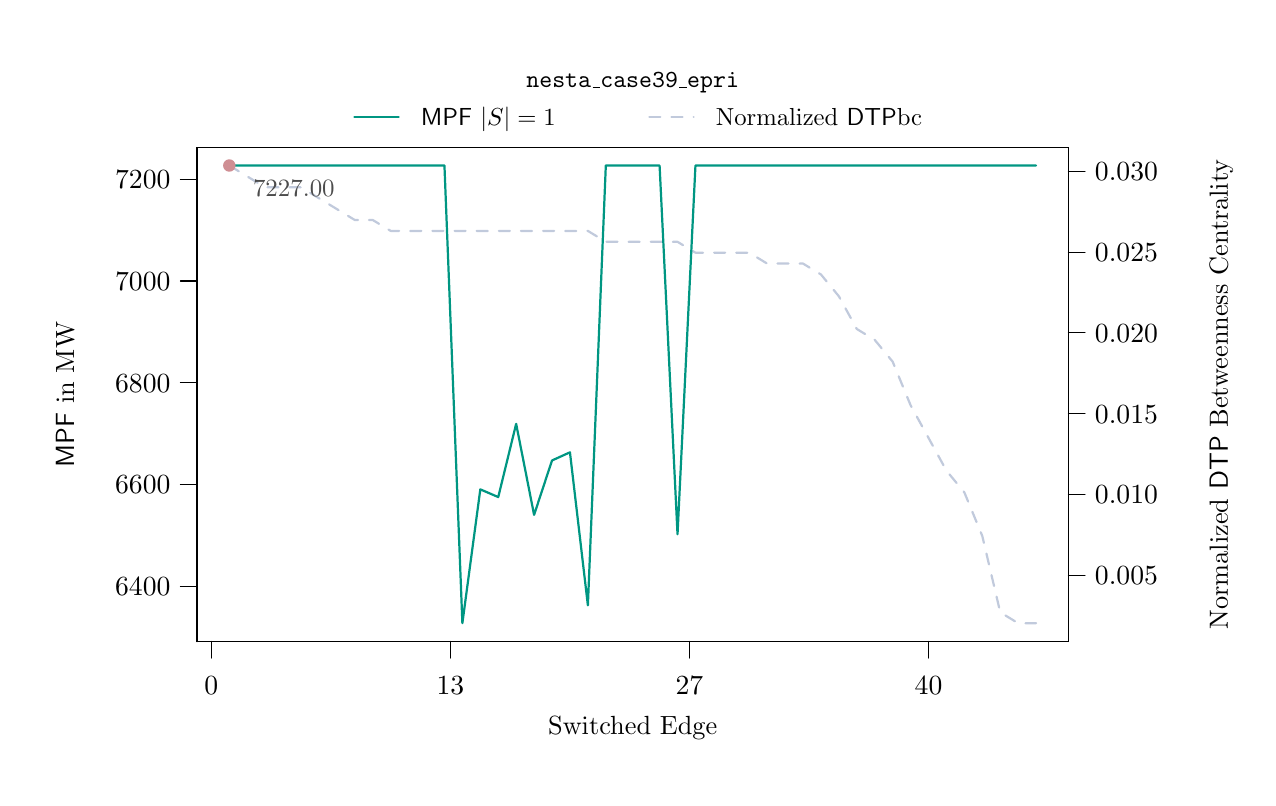
\begin{tikzpicture}[x=1pt,y=1pt]
\definecolor{fillColor}{RGB}{255,255,255}
\path[use as bounding box,fill=fillColor,fill opacity=0.00] (0,0) rectangle (440.85,271.01);
\begin{scope}
\path[clip] (  0.00,  0.00) rectangle (440.85,271.01);
\definecolor{drawColor}{RGB}{193,202,220}

\path[draw=drawColor,line width= 0.8pt,dash pattern=on 4pt off 4pt ,line join=round,line cap=round] ( 72.86,221.20) --
	( 79.34,217.26) --
	( 85.82,213.32) --
	( 92.30,213.32) --
	( 98.77,213.32) --
	(105.25,209.38) --
	(111.73,205.45) --
	(118.21,201.51) --
	(124.69,201.51) --
	(131.17,197.57) --
	(137.64,197.57) --
	(144.12,197.57) --
	(150.60,197.57) --
	(157.08,197.57) --
	(163.56,197.57) --
	(170.04,197.57) --
	(176.51,197.57) --
	(182.99,197.57) --
	(189.47,197.57) --
	(195.95,197.57) --
	(202.43,197.57) --
	(208.91,193.63) --
	(215.38,193.63) --
	(221.86,193.63) --
	(228.34,193.63) --
	(234.82,193.63) --
	(241.30,189.70) --
	(247.78,189.70) --
	(254.25,189.70) --
	(260.73,189.70) --
	(267.21,185.76) --
	(273.69,185.76) --
	(280.17,185.76) --
	(286.65,181.82) --
	(293.12,173.95) --
	(299.60,162.13) --
	(306.08,158.19) --
	(312.56,150.32) --
	(319.04,134.57) --
	(325.52,122.76) --
	(331.99,110.94) --
	(338.47,103.07) --
	(344.95, 87.32) --
	(351.43, 59.75) --
	(357.91, 55.82) --
	(364.39, 55.82);
\end{scope}
\begin{scope}
\path[clip] (  0.00,  0.00) rectangle (440.85,271.01);
\definecolor{drawColor}{RGB}{0,0,0}

\path[draw=drawColor,line width= 0.4pt,line join=round,line cap=round] ( 61.20, 49.20) --
	(376.05, 49.20) --
	(376.05,227.81) --
	( 61.20,227.81) --
	( 61.20, 49.20);
\end{scope}
\begin{scope}
\path[clip] (  0.00,  0.00) rectangle (440.85,271.01);
\definecolor{drawColor}{RGB}{0,0,0}

\path[draw=drawColor,line width= 0.4pt,line join=round,line cap=round] (376.05, 73.18) -- (376.05,219.07);

\path[draw=drawColor,line width= 0.4pt,line join=round,line cap=round] (376.05, 73.18) -- (382.05, 73.18);

\path[draw=drawColor,line width= 0.4pt,line join=round,line cap=round] (376.05,102.36) -- (382.05,102.36);

\path[draw=drawColor,line width= 0.4pt,line join=round,line cap=round] (376.05,131.54) -- (382.05,131.54);

\path[draw=drawColor,line width= 0.4pt,line join=round,line cap=round] (376.05,160.71) -- (382.05,160.71);

\path[draw=drawColor,line width= 0.4pt,line join=round,line cap=round] (376.05,189.89) -- (382.05,189.89);

\path[draw=drawColor,line width= 0.4pt,line join=round,line cap=round] (376.05,219.07) -- (382.05,219.07);

\node[text=drawColor,anchor=base west,inner sep=0pt, outer sep=0pt, scale=  1.00] at (385.65, 69.74) {0.005};

\node[text=drawColor,anchor=base west,inner sep=0pt, outer sep=0pt, scale=  1.00] at (385.65, 98.91) {0.010};

\node[text=drawColor,anchor=base west,inner sep=0pt, outer sep=0pt, scale=  1.00] at (385.65,128.09) {0.015};

\node[text=drawColor,anchor=base west,inner sep=0pt, outer sep=0pt, scale=  1.00] at (385.65,157.27) {0.020};

\node[text=drawColor,anchor=base west,inner sep=0pt, outer sep=0pt, scale=  1.00] at (385.65,186.45) {0.025};

\node[text=drawColor,anchor=base west,inner sep=0pt, outer sep=0pt, scale=  1.00] at (385.65,215.63) {0.030};
\end{scope}
\begin{scope}
\path[clip] (  0.00,  0.00) rectangle (440.85,271.01);
\definecolor{drawColor}{RGB}{0,150,130}

\path[draw=drawColor,line width= 0.8pt,line join=round,line cap=round] ( 72.86,221.20) --
	( 79.34,221.20) --
	( 85.82,221.20) --
	( 92.30,221.20) --
	( 98.77,221.20) --
	(105.25,221.20) --
	(111.73,221.20) --
	(118.21,221.20) --
	(124.69,221.20) --
	(131.17,221.20) --
	(137.64,221.20) --
	(144.12,221.20) --
	(150.60,221.20) --
	(157.08, 55.82) --
	(163.56,104.18) --
	(170.04,101.39) --
	(176.51,127.85) --
	(182.99, 94.96) --
	(189.47,114.62) --
	(195.95,117.56) --
	(202.43, 62.25) --
	(208.91,221.20) --
	(215.38,221.20) --
	(221.86,221.20) --
	(228.34,221.20) --
	(234.82, 87.97) --
	(241.30,221.20) --
	(247.78,221.20) --
	(254.25,221.20) --
	(260.73,221.20) --
	(267.21,221.20) --
	(273.69,221.20) --
	(280.17,221.20) --
	(286.65,221.20) --
	(293.12,221.20) --
	(299.60,221.20) --
	(306.08,221.20) --
	(312.56,221.20) --
	(319.04,221.20) --
	(325.52,221.20) --
	(331.99,221.20) --
	(338.47,221.20) --
	(344.95,221.20) --
	(351.43,221.20) --
	(357.91,221.20) --
	(364.39,221.20);
\end{scope}
\begin{scope}
\path[clip] (  0.00,  0.00) rectangle (440.85,271.01);
\definecolor{drawColor}{RGB}{0,0,0}

\path[draw=drawColor,line width= 0.4pt,line join=round,line cap=round] ( 61.20, 49.20) --
	(376.05, 49.20) --
	(376.05,227.81) --
	( 61.20,227.81) --
	( 61.20, 49.20);
\end{scope}
\begin{scope}
\path[clip] (  0.00,  0.00) rectangle (440.85,271.01);
\definecolor{drawColor}{RGB}{0,0,0}

\path[draw=drawColor,line width= 0.4pt,line join=round,line cap=round] ( 61.20, 69.23) -- ( 61.20,216.24);

\path[draw=drawColor,line width= 0.4pt,line join=round,line cap=round] ( 61.20, 69.23) -- ( 55.20, 69.23);

\path[draw=drawColor,line width= 0.4pt,line join=round,line cap=round] ( 61.20,105.98) -- ( 55.20,105.98);

\path[draw=drawColor,line width= 0.4pt,line join=round,line cap=round] ( 61.20,142.73) -- ( 55.20,142.73);

\path[draw=drawColor,line width= 0.4pt,line join=round,line cap=round] ( 61.20,179.48) -- ( 55.20,179.48);

\path[draw=drawColor,line width= 0.4pt,line join=round,line cap=round] ( 61.20,216.24) -- ( 55.20,216.24);

\node[text=drawColor,anchor=base east,inner sep=0pt, outer sep=0pt, scale=  1.00] at ( 51.60, 65.79) {6400};

\node[text=drawColor,anchor=base east,inner sep=0pt, outer sep=0pt, scale=  1.00] at ( 51.60,102.54) {6600};

\node[text=drawColor,anchor=base east,inner sep=0pt, outer sep=0pt, scale=  1.00] at ( 51.60,139.29) {6800};

\node[text=drawColor,anchor=base east,inner sep=0pt, outer sep=0pt, scale=  1.00] at ( 51.60,176.04) {7000};

\node[text=drawColor,anchor=base east,inner sep=0pt, outer sep=0pt, scale=  1.00] at ( 51.60,212.79) {7200};
\end{scope}
\begin{scope}
\path[clip] (  0.00,  0.00) rectangle (440.85,271.01);
\definecolor{fillColor}{RGB}{207,142,147}

\path[fill=fillColor] ( 72.86,221.20) circle (  2.25);
\end{scope}
\begin{scope}
\path[clip] (  0.00,  0.00) rectangle (440.85,271.01);
\definecolor{drawColor}{RGB}{0,0,0}

\path[draw=drawColor,line width= 0.4pt,line join=round,line cap=round] ( 61.20, 49.20) --
	(376.05, 49.20) --
	(376.05,227.81) --
	( 61.20,227.81) --
	( 61.20, 49.20);
\end{scope}
\begin{scope}
\path[clip] (  0.00,  0.00) rectangle (440.85,271.01);
\definecolor{drawColor}{gray}{0.30}

\node[text=drawColor,anchor=base,inner sep=0pt, outer sep=0pt, scale=  0.90] at ( 96.18,210.04) {7227.00};
\end{scope}
\begin{scope}
\path[clip] (  0.00,  0.00) rectangle (440.85,271.01);
\definecolor{drawColor}{RGB}{0,0,0}

\path[draw=drawColor,line width= 0.4pt,line join=round,line cap=round] ( 66.38, 49.20) -- (325.52, 49.20);

\path[draw=drawColor,line width= 0.4pt,line join=round,line cap=round] ( 66.38, 49.20) -- ( 66.38, 43.20);

\path[draw=drawColor,line width= 0.4pt,line join=round,line cap=round] (152.76, 49.20) -- (152.76, 43.20);

\path[draw=drawColor,line width= 0.4pt,line join=round,line cap=round] (239.14, 49.20) -- (239.14, 43.20);

\path[draw=drawColor,line width= 0.4pt,line join=round,line cap=round] (325.52, 49.20) -- (325.52, 43.20);

\node[text=drawColor,anchor=base,inner sep=0pt, outer sep=0pt, scale=  1.00] at ( 66.38, 30.00) {0};

\node[text=drawColor,anchor=base,inner sep=0pt, outer sep=0pt, scale=  1.00] at (152.76, 30.00) {13};

\node[text=drawColor,anchor=base,inner sep=0pt, outer sep=0pt, scale=  1.00] at (239.14, 30.00) {27};

\node[text=drawColor,anchor=base,inner sep=0pt, outer sep=0pt, scale=  1.00] at (325.52, 30.00) {40};

\node[text=drawColor,anchor=base,inner sep=0pt, outer sep=0pt, scale=  0.95] at (218.62, 15.60) {Switched Edge};

\node[text=drawColor,rotate= 90.00,anchor=base,inner sep=0pt, outer sep=0pt, scale=  0.95] at ( 16.80,138.51) {$\mathsf{MPF}$ in~$\mathrm{MW}$};

\node[text=drawColor,rotate= 90.00,anchor=base,inner sep=0pt, outer sep=0pt, scale=  0.95] at (433.65,138.51) {Normalized~$\mathsf{DTP}$ Betweenness Centrality};
\end{scope}
\begin{scope}
\path[clip] (  0.00,  0.00) rectangle (440.85,271.01);
\definecolor{drawColor}{RGB}{0,150,130}

\path[draw=drawColor,line width= 0.8pt,line join=round,line cap=round] (118.04,238.60) -- (134.06,238.60);
\definecolor{drawColor}{RGB}{193,202,220}

\path[draw=drawColor,line width= 0.8pt,dash pattern=on 4pt off 4pt ,line join=round,line cap=round] (224.63,238.60) -- (240.65,238.60);
\definecolor{drawColor}{RGB}{0,0,0}

\node[text=drawColor,anchor=base,inner sep=0pt, outer sep=0pt, scale=  0.89] at (218.62,249.28) {\texttt{nesta\_case39\_epri}};

\node[text=drawColor,anchor=base west,inner sep=0pt, outer sep=0pt, scale=  0.89] at (142.07,235.54) {$\mathsf{MPF}~|S|=1$};

\node[text=drawColor,anchor=base west,inner sep=0pt, outer sep=0pt, scale=  0.89] at (248.66,235.54) {Normalized~$\mathsf{DTP}$bc};
\end{scope}
\end{tikzpicture}
